\chapter{Functions}

\section{Sets}
Before defining what a function is or what it does, it is important to briefly discuss what goes into function and what comes out. Simply, \textit{sets}\index{set} are a collection of items and each one of those items are usually referred to as \textit{elements}\index{set!element}. Without getting into the weeds of set theory, sets can contain pretty much anything from numbers, functions, and other sets \cite{bookofproof}.

Some common sets that you may be familiar with are the \textit{natural numbers} $\N = \{1,2,3,4,5,\dots\}$, the \textit{integers} $\Z = \{\dots,-2,-1,0,1,2,\dots\}$, and the \textit{real numbers} $\R$, which is usually represented via a number line. Sets can also be intervals on the real line (i.e. [a,b) is an interval on $\R$ containing $a$ but not $b$) or even the possible results of flipping a coin $C = \{H,T\}$.

We will now define the basic notation when dealing with sets and the operations that can be performed on sets. We say that $x$ is an element of a set $A$ with the notation $x \in A$ and when $x$ is not in $A$, we say $x \not\in A$. For example, given the set $A = \{1,2,3,4\}$, we can say that $1 \in A$ is true as well as $5 \not\in A$.

The notion of combining sets comes with \textit{unions}\index{set!union} and \textit{intersections}\index{set!intersection}. Given $A$ and $B$ are sets, the union of $A$ and $B$ is denoted as $A \cup B$ and is equal to the set the contains elements in either $A$ or $B$. Similarly, the intersection between $A$ and $B$ is denoted as $A \cap B$ and is the set that contains elements that are in both $A$ and $B$. For example, given the sets $A = \{1,2,3,4\}$ and $B = \{3,4,5,6\}$, the union and intersection between $A$ and $B$ is

\begin{aequation}
    A \cup B &= \{1,2,3,4,5,6\} \\
    A \cap B &= \{3,4\}
\end{aequation}

Subsets are often used to relate different sets and their elements. A set $A$ is said to be a subset of another set $B$ if all of the elements of $A$ are also within $B$ and is denoted as $A \subseteq B$ and a set $A$ is equal to a set $B$ if and only if $A \subseteq B$ and $B \subseteq A$. An important subset is the empty set represented by the symbols $\varnothing$, $\emptyset$, or simply $\{\}$. It is important to note that the empty set is also a subset of all sets.

Using sets by listing them out can become cumbersome and sometimes confusing, instead set builder notation is used to build a set based on a rule. For example, the set of all positive even integers can be written as

\begin{equation}
    A = \{2,4,6,8,\dots\} = \{z : z \text{ is an positive even integer}\} = \{z : z = 2n, n\in\Z \text{ and } n > 0\}
\end{equation}

\noindent Here, the $:$ stands for "such that" which indicates the rule (the words "such that" or the symbol $|$ is also often used). The \textit{rational numbers} $\Q$ can also be constructed via the integers with

\begin{equation}
    \Q = \{\frac{p}{q} : p,q \in \Z \text{ and } q \neq 0\}
\end{equation}

As mentioned previously, intervals on the real number line can be represented as sets. Given two values $a$ and $b$ and assuming that $a \leq b$, intervals on the real line are represented as

\begin{itemize}
    \item Closed interval: $[a,b] = \{x \in \R : a \leq x \leq b\}$ \hfill \intervalinline{a}{b}{[}{]}
    \item Open interval: $(a,b) = \{x \in \R : a < x < b\}$ \hfill \intervalinline{a}{b}{(}{)}
    \item Half-open interval:
        \begin{itemize}
            \item $(a,b] = \{x \in \R : a < x \leq b\}$ \hfill \intervalinline{a}{b}{(}{]}
            \item $[a,b) = \{x \in \R : a \leq x < b\}$ \hfill \intervalinline{a}{b}{[}{)}
        \end{itemize}
    \item Infinite interval:
        \begin{itemize}
            \item $(a,\infty) = \{x \in \R: a < x\}$ \hfill \intervalinline{a}{$\infty$}{(}{}
                \item $[a,\infty) = \{x \in \R: a \leq x\}$ \hfill \intervalinline{a}{$\infty$}{[}{}
                \item $(-\infty,b) = \{x \in \R: x < b\}$ \hfill \intervalinline{$-\infty$}{b}{}{)}
            \item $(-\infty,b] = \{x \in \R: x \leq b\}$ \hfill \intervalinline{$-\infty$}{b}{}{]}
            \item $(-\infty,\infty) = \R$ \hfill \intervalinline{$-\infty$}{$\infty$}{}{}
        \end{itemize}
\end{itemize}

\noindent Here, the open brackets $($ and $)$ indicate that the respective endpoint is not included, while the closed brackets $[$ and $]$ indicate that the respective endpoint is included in the interval.

The \textit{Cartesian product}\index{set!Cartesian product} (also known as the \textit{direct product}\index{set!direct product}) is used often to describe ordered pairs or even higher-dimension coordinates. Some examples include the $xy$-plane also known as $\R^2$, 3D space with $\R^3$. The Cartesian product for two sets $A$ and $B$ is defined as

\begin{equation}
    A \times B = \{(a,b) : a \in A, b \in B\}
\end{equation}

\noindent Note that, in general, $A \times B \neq B \times A$ as the operation is order dependent. Higher-order products are defined with sets $A_1, A_2, \dots, A_n$ as

\begin{equation}
    A_1 \times A_2 \times \cdots \times A_n = \{(a_1,a_2,\dots,a_n): a_i \in A_i, i \in \{1,2,\dots,n\}\}
\end{equation}

\noindent As previously mentioned, the 2D plane as well as the 3D plane can be constructed using Cartesian products as well and is done as such with the set of real numbers $\R$

\begin{aequation}
    \R^2 &= \R \times \R = \{(x,y): x,y \in \R\}\\
    \R^3 &= \R \times \R \times \R = \{(x,y,z): x,y,z \in \R\}\\
    & \vdots \\
    \R^n &= \R \times \R \times \dots \times \R = \{(x_1, x_2, \dots, x_n) : x_i \in \R, i \in \{1,2,\dots, n\} \}
\end{aequation}

For further and more formal discussion on sets and naive set theory as well as formal logic and proof writing, refer to \cite{naivesettheory} or \cite{bookofproof}.

\section{What is a function?}
\textit{Functions}\index{function} are objects in math that describe a relationship or mapping between two sets. Given two sets $X$ and $Y$, a function $f$ maps the unique elements of $X$, called the \textit{domain}\index{function!domain} of the function, to elements in the set $Y$ called the \textit{codomain}\index{function!codomain} of the function and the relationship is denoted as $f : X \to Y$ ("$f$ maps from $X$ to $Y$") or $y = f(x)$ ("$y$ equals $f$ of $x$" \cite{understandinganalysis}), where $y \in R \subseteq Y$ is known as the \textit{dependent variable}\index{function!dependent variable} with $R$ as the range of the function and $x \in X$ is known as the \textit{independent variable}\index{function!independent variable} or the \textit{argument}\index{function!argument} of the function. The \textit{range}\index{function!range} of a function is the set of all possible values that $f(x)$ is able to output with $X$ as its domain, note that the range is a subset of the codomain $Y$ but is not always equal. Formally, the definition is as follows

\begin{definition}
    A \textit{function} is a mapping or rule that assigns each element from a set called the domain $X$ of the function to a unique element in the range $R = f(X)$ of the function which is a subset of the codomain $R \subseteq Y$ and the element $x \in X$ is mapped to an element in $y \in R \subseteq Y$ with $x \mapsto y$.
\end{definition}

Further emphasis must be made on the elements $y = f(x)$. The function $f(x)$ maps the element $x \in X$ to exactly one element $y \in Y$ \cite{elemrealandcomplex}. For single variable functions, this can be tested using the vertical line test on a function's graph (covered shortly). If a formula results in two answers with one input (i.e. the equation for a circle: $x^2 + y^2 = r$ gives two points of $y$ for each $x$) it is no longer considered a function. Figure \ref{functionmapping} shows how a function maps elements of the domain to the range.

\begin{figure}[!ht]
    \centering
    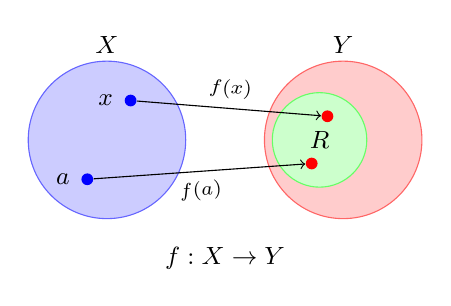
\begin{tikzpicture}[font=\small]
        % % Origin (for reference)
        % \node (origin) at (0,0) {$\bullet$};

        % Domain (X) - Blue circle
        \filldraw[fill=blue!20, draw=blue!60] (-1.5,0) circle (1cm);
        \node at (-1.5,1.2) {$X$};  % Domain label above circle

        % Codomain (Y) - Red circle with Range (R) - Green circle
        \filldraw[fill=red!20, draw=red!60] (1.5,0) circle (1cm);
        \node at (1.5,1.2) {$Y$};  % Codomain label above circle
        \filldraw[fill=green!20, draw=green!60] (1.2,0) circle (0.6cm);
        \node at (1.2,0) {$R$};  % Range label centered in green circle

        % Domain points with tight labels
        \node[circle,fill=blue,inner sep=1.5pt] (x) at (-1.2,0.5) {};
        \node[left=0.1cm] at (x) {$x$};

        \node[circle,fill=blue,inner sep=1.5pt] (a) at (-1.75,-0.5) {};
        \node[left=0.1cm] at (a) {$a$};

        % Codomain points
        \node[circle,fill=red,inner sep=1.5pt] (fx) at (1.3,0.3) {};
        \node[circle,fill=red,inner sep=1.5pt] (fa) at (1.1,-0.3) {};

        % Arrows with labels attached
        \draw[->] (x) -- node[midway,above,sloped] {\scriptsize$f(x)$} (fx);
        \draw[->] (a) -- node[midway,below,sloped] {\scriptsize$f(a)$} (fa);

        % Function label below
        \node at (0,-1.5) {$f: X \to Y$};
    \end{tikzpicture}
    \caption{Function mapping diagram showing the domain $X$, codomain $Y$, and range $f(X)$}
    \label{functionmapping}
\end{figure}

\begin{example}
    Some real-world examples of functions are
    \begin{itemize}
        \item The area of a circle: \dotfill $A(r) = \pi r^2$
        \item The height of a falling ball: \dotfill $h(t) = h_0 + v_0 t - (1/2)gt^2$
        \item Compound interest: \dotfill $A(t) = P(1+\frac{r}{n})^{nt}$
        \item Temperature conversion: \dotfill $C(F) = \frac{5}{9}(F - 32)$
        \item %TODO: add more examples here
    \end{itemize}
    It can be useful to think of functions as machines that take in an input and produces an output. The examples above show such cases using mathematical formulas that give a set of instructions on how the input is transformed from the element in the domain to the element in the range.
\end{example}

Another way to represent functions is with its \textit{graph}\index{function!graph} which is a set of points consisting of the input and its corresponding output and is represented with the set of ordered pairs $\{(x,y) : y = f(x), x\in\R\}$ for functions that accept real numbers.

\begin{example}
    A familiar example is the linear function $f(x) = mx + b$ where $m$ is the slope of the line and $b$ is the vertical offset. Suppose $m = 1$ and $b = 0$, we get the following graph for the function $f(x) = x$ in figure \ref{f(x)=x graph}
    \begin{figure}[!ht]
        \centering
        \begin{tikzpicture}
            \begin{axis}[xmin=-2, xmax=2, ymin=-2, ymax=2,
                axis lines=middle, xlabel=$x$, ylabel=$y$]
                \addplot[color=black,grid,]{x};
            \end{axis}
        \end{tikzpicture}
        \label{f(x)=x graph}
        \caption{Graph of the function $f(x) = x$}
    \end{figure}
\end{example}

\begin{example}
    Another example is the quadratic function of the form $f(x) = ax^2 + bx + c$, where $a,b,c \in \R$ are the coefficients of the function and determine its shape. Suppose that $a = 1, b = 0, c = -1$ resulting in the function $f(x) = x^2 - 1$. Using knowledge of the roots a quadratic function, it can be deduced that this will result in a parabola with $x$-intersections at $x = -1$ and $x = 1$ which can be confirmed in the graph in figure \ref{f(x)=x^2-1graph}

    \begin{figure}[!ht]
        \centering
        \begin{tikzpicture}
            \begin{axis}[
                    xmin=-2, xmax=2,
                    ymin=-2, ymax=2,
                    xlabel=$x$, ylabel=$y$,
                    axis lines=middle,
                    % grid=both
                ]
                \addplot[color=black, domain=-2:2, samples=50]{x^2 - 1};
            \end{axis}
        \end{tikzpicture}
        \label{f(x)=x^2-1graph}
        \caption{Graph of the function $f(x) = x^2-1$}
    \end{figure}
\end{example}

\section{Common Functions}

\section{Types of Functions}
\subsection{Even and Odd Functions}
\subsection{Increasing and Decreasing Functions}
\subsection{Periodic Functions}

\section{Inverse Function}

\section{Function Compositions}

\section{Function Transformations and Operations}
